\label{sec:algorithm}

%Proposed method combines several useful concepts, that allows it to be applied for wide range of real-world problems. 
Let $(\P(\theta), \theta \in \Theta \subseteq \mathbb{R}^p)$ be a parametric assumption about observed data $\mathbb{Y} = (Y_1,...,Y_N)$.
For structural break detection the algorithm uses the likelihood-ratio test statistic (LRT) in a rolling window.
Let $2h$ be a size of the rolling window and $t$ be a candidate for a change point, $1 + h \leq t \leq N - h + 1$, then 
the hypothesis testing problem can be stated as follows:

\[H_0: \{Y_i\}_{i = t - h}^{t - 1} \backsim ~\P_1, ~ \{Y_i\}_{i = t}^{t + h - 1} \backsim~ \P_2
\]
\[
H_1: \{Y_i\}_{i=t - h}^{t + h - 1} \backsim ~\P_1,
\]
where $\P_1 = \P(\theta^*_1)$, $\P_2 = \P(\theta^*_2)$, and $\theta^*_1, \theta^*_2 \in \Theta$.
A possible solution is likelihood-ratio test \citet{GLR_Siegm}, \citet{LRTWilks}, \citet{nonParamMLE}: 

\[
T_{h}(t) = \sup_{\theta \in \Theta}L(\theta; Y_{t-h},..., Y_{t-1}) + \sup_{\theta \in \Theta}L(\theta; Y_{t},...,
Y_{t+h-1})
\]
\[
-\sup_{\theta \in \Theta}\{L(\theta; Y_{t-h},..., Y_{t-1}) + L(\theta; Y_{t},..., Y_{t+h-1})\},
\]
$L(\theta;\cdot)$ is a log-likelihood function.

%Under the assumptions \ref{cond_A}, \ref{cond_L_star},  that of parametric family, the statistic $T_h(\cdot)$ behaves as a non-central $\chi^2_p$ distribution if hypothesis $H_0$ is correct and like $\chi^2_p$ under its alternative. $p$ is the size of parameter space $\mathbb{R}^p$.

%Under some assumptions on geometric properties of the parametric family  $(\P(\theta)$, 
The statistic $T_h(\cdot)$ behaves as the one having a non-central $\chi^2_p$ distribution if the hypothesis $H_0$ is not rejected. Otherwise, $T_h(\cdot)$ is distributed as $\chi^2_p$, where $p$ is a dimension of the parametric space. 

\begin{proposition}
\label{prop1}
Under conditions \ref{cond_A}, \ref{cond_L_star}, it is hold with probability $1 - 4 e^{-x}$, that 
\[
|\sqrt{2 T_h(t)} - \Vert  \xi_t + b_h(t)\Vert|  \leq 10 \diamondsuit (r, x),
\]
where $\xi_t \backsim \mathcal{N}(0, I_p)$, $I_p$ is an identity matrix,
\[
  b_h(t) = \begin{cases}
    \Sigma_h|\theta_1^* - \theta_2^*|, & \text{if $H_0$},\\
     $0$ , & \text{if $H_1$};
  \end{cases}
\]

$b_{h}(t)$ is a systematic drift component; $\Sigma$ is a positive matrix, $\theta_1^*$ and $\theta_2^*$  are target parameters before and after the structural change respectively.
\end{proposition}  
Proposition~\ref{prop1} is proved in Section~\ref{sec:theory}.\\

% has a none-zero value, if a change point $\tau$ is inside of the rolling window, $\tau \in \{t-h,...,t+h\}$ 
Instead of analysing a single value of the statistic $T_h(t)$ at a single point of interest $t$, we do so for all points inside of a running window: $\mathbb{T}_{h}(t) = (T_{h}(t - h),..., T_{h}(t + h - 1))$. The vector $\mathbb{T}_{h}(t)$ has the same 
geometric properties as a vector $\mathbb{b}_{h}(t) = (b_{h}(t - h),..., b_{h}(t + h - 1))$ has. This vector forms a type of a pattern depending on a type of a change. It is referred to as a \textit{change-point-pattern}. Several illustrations of the concept are presented in Fig.\ref{fig:triang1} - \ref{fig:triang2}.

\begin{figure}[!h]
    \centering
    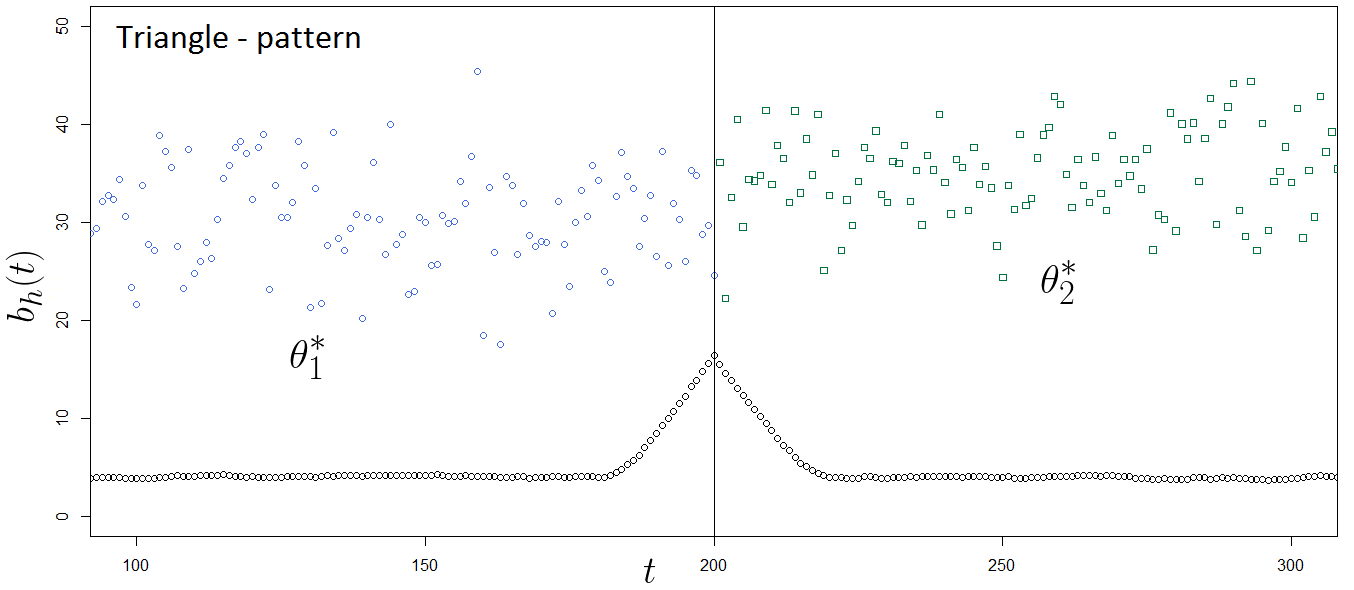
\includegraphics[width=0.4\textwidth, height=0.2\textwidth]{images/pat3.png}
    \caption{Behaviour of $b_{h}(t)$ in case of abrupt change point}
    \label{fig:triang1}
\end{figure}

\begin{figure}[!h]
    \centering
    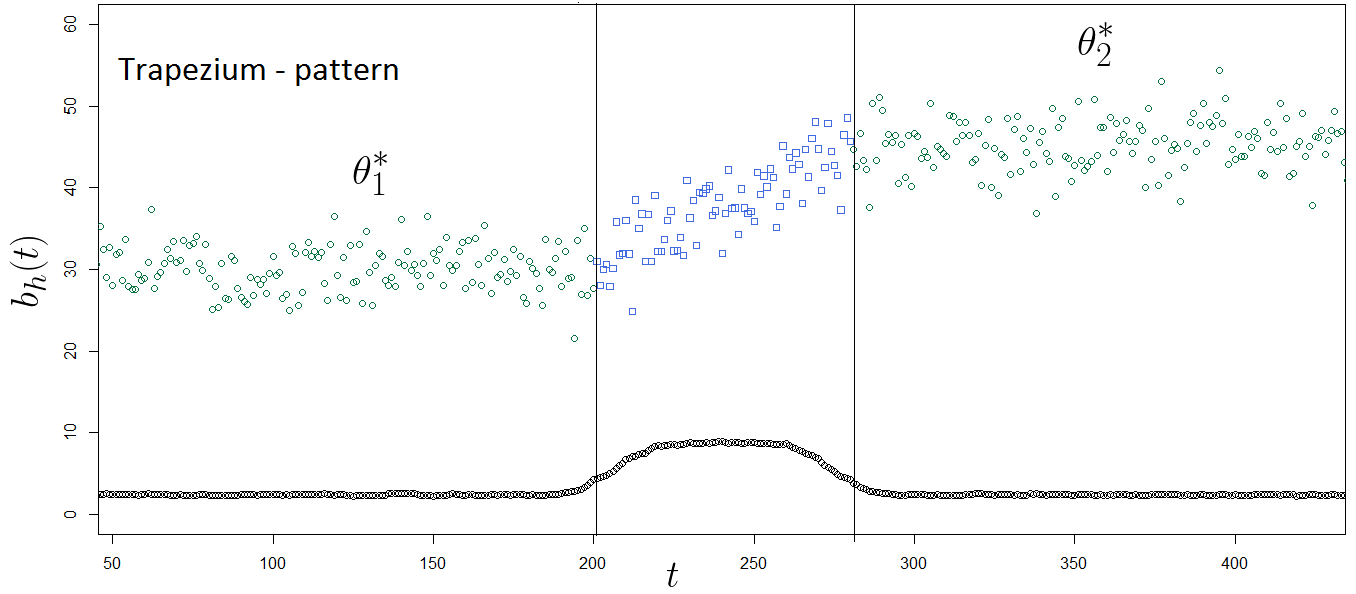
\includegraphics[width=0.4\textwidth, height=0.2\textwidth]{images/pat2.png}
    \caption{Behaviour of $b_{h}(t)$ in case of smooth transition}
    \label{fig:trap}
\end{figure}

\begin{figure}[!h]
    \centering
    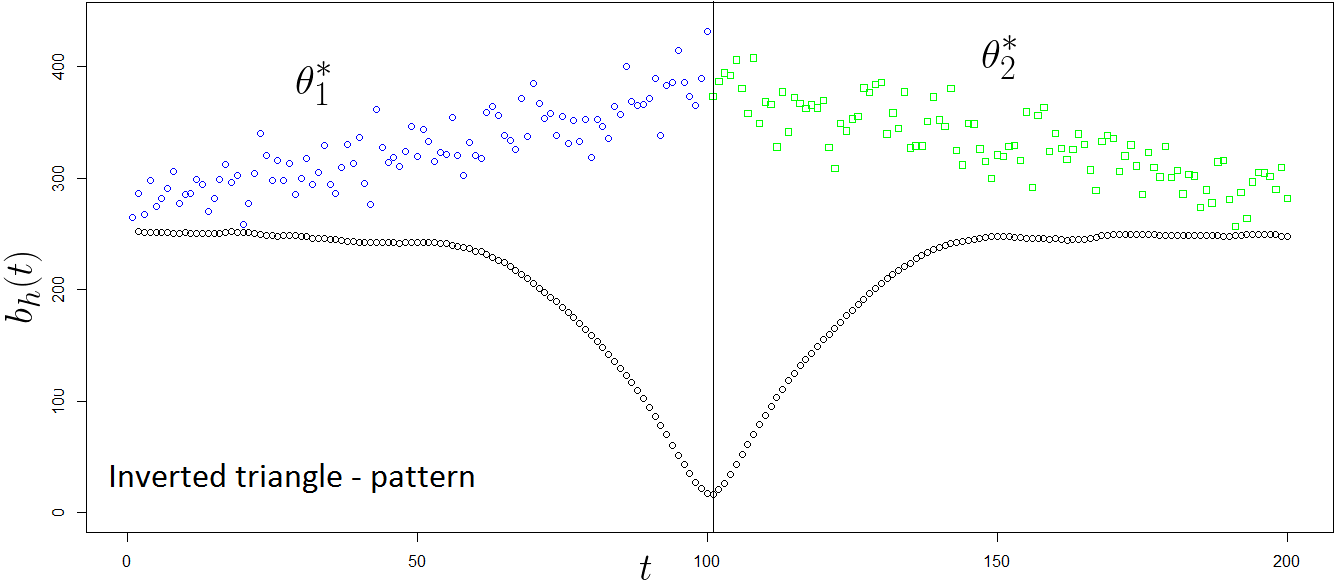
\includegraphics[width=0.4\textwidth, height=0.2\textwidth]{images/pat1-1.png}
    \caption{Behaviour of $b_{h}(t)$ in case of break in trend}
    \label{fig:triang2}
\end{figure}


The Fig.\ref{fig:triang1} shows a triangle pattern. It is produced by an abrupt change in a parameter of an observed signal. The jump takes place at the moment $t = 200$. Until that moment, the signal is distributed according to $\P(\theta^*_1) = N(30, 5)$ and after the jump it is obeyed to $\P(\theta^*_2) = N(35, 5)$, $\theta_1^* = 30$, $\theta_2^* = 35$.
A smooth transition from $\theta_1^*$ to $\theta_2^*$ leads to the formation of trapezium pattern. In Fig.\ref{fig:trap} is presented the transition between two Gaussian random processes: from $N(30, 5)$ to $N(45, 5)$, $\theta_1^* = 30$, $\theta_2^* = 45$.
The last pattern (Fig.\ref{fig:triang2}) is an inverted triangle. It appears because of a change point in a piece-wise linear regression model. Namely, $Y_i = i + \eps_i$ before the change point and  $Y_i = (-i + 100) + \eps_i$ after the change point, where $\eps_i \backsim N(0, 25)$ is normally distributed homogeneous noise. \\
%So that to be more robust for outliers, algorithm monitors  $\hat{T}_{h}(t)$, rather than $T_{h}(t)$. 

%The minimum size $2h_{min}$ of running window, at which pattern becomes distinguishable is called optimal window size. 
The distinguishability of the change point pattern depends on the window size $2h$ and the size of a change point $|\theta_1^* - \theta_2^*|$. In other words, for each size of a change point exists the optimal scale $h_{opt}$, s.t. for each $h < h_{opt}$ the pattern is poorly visualised.   
The detailed description of the $h_{opt}$-concept can be found in Section \ref{subsec:win_size}. An example is presented in Fig.\ref{fig:scales}. Gaussian data with abrupt change in mean at the moment $\tau = 342$ is depicted at the first line. The next two panels show test statistics $ T_{2h = 4}(t)$ and $T_{2h = 10}(t)$ respectively. In both cases the change point pattern is still uncertain. The last test statistic $T_{2h = 20}(t)$ forms a distinguishable triangle. For this example $5 < h_{opt} \leq 10$. 
\begin{figure}[!h]
    \centering
    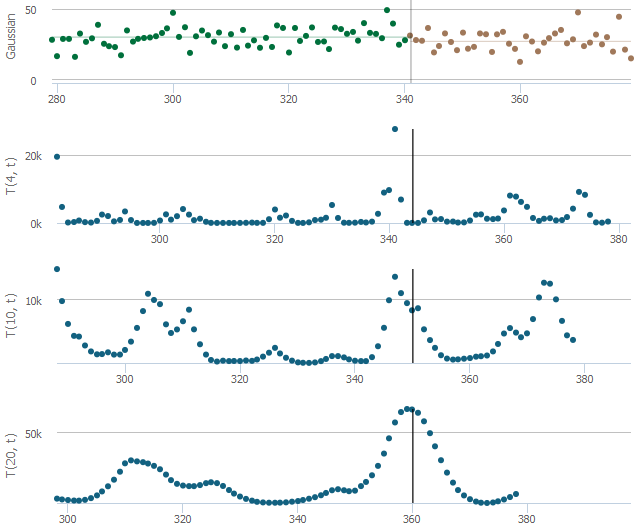
\includegraphics[width=0.4\textwidth, height=0.4\textwidth]{images/multiscale.png}
    \caption{Pattern on different scales}
    \label{fig:scales}
\end{figure}
The procedure monitors not the changes in statistic $T_{h}(t)$ itself, but in its convolution with a target \textit{change-point pattern} $P_{h}$. This makes algorithm less sensitive for outliers.
\[
\hat{T}_{h}(t) = \langle\mathbb{T}_{h}(t), P_{h}\rangle
\]
where
\[
\mathbb{T}_{h}(t) = (T_{h}(t - h),..., T_{h}(t + h - 1)). 
\]
Abrupt change in an observed parameter entails triangle-like behaviour of test statistics $T_{h}(\cdot)$. Therefore, in this case the target pattern $P_h$ is an isoscales triangle with a unit height and a base equal to $2h$.

Naturally, the most desirable way is to use only the smallest window $2h_{opt}$. In practice, it is not possible, as it was mentioned before, $2h_{opt}$ depends on parameters before and after structural break: $h_{opt} = h_{opt}(\theta_1^*, \theta_2^*)$. Here we propose a \textit{multiscale} approach. It implies that the statistic $\hat{T}_{h}(t)$ is computed simultaneously in running windows of different sizes $H = (h_1,..., h_n)$. This allows algorithm to estimate the smallest window size $2h_{opt}$ automatically: exists $h_k \in H$, s.t. $h_k < h_{opt} \leq h_{k+1} $. Critical values $\{z(h)\}_{h \in H}$ for $\{\hat{T}_{h}(\cdot)\}$ are computed using the multiplier bootstrap. Under this approach, introduction of multiscality entails the problem of multiplicity correction. To overcome it we use \text{synchronisation} technique. The detailed description of the multiplier bootstrap procedure and the synchronisation are presented in \citet{SpokoinyBoot}. 

The presented algorithm can be applied for both sequential and retrospective settings. Under \textit{online} framework, it marks a time moment $\tau$ as a change point,  if test statistics $\hat{T}_{h}(\tau + h)$ exceeds critical value $z(h)$ at the moment $\tau + h$:
\[
\{\tau: \hat{T}_{h}(\tau - h) > z(h)\}.
\]
This means, that the smallest delay of detection is $h_{min}$.

Under \textit{offline} setting, $\tau$ is a change point if
\[
\{\tau = \argmax_{t \in \{1,...,N\}} \hat{T}_{h}(t)\}.
\]

The greater number $k$ of such scales $h'_{i_1},...,h'_{i_k}$  where $\tau$ is marked as change point, the more sure algorithm is, that $\tau$ the \textit{true} change point is.



%A moment $\tau$ is marked as a \textit{candidate} for a change point, if exists a scale $h'_i$, s.t. the value of $\hat{T}_{h'_i}(\tau)$ overcomes critical value:
%\[
%\hat{T}_{h'_i}(\tau) > z(h'_i).
%\]

%Procedure of change point detection is repeated at each scale $h \in H$. $\{h_i\}$, 


%\textcolor{red}{[TODO:Explain mathematical idea of patterns]}
%The size of a pattern obviously depends on size of sliding window. To make method more robust for outliers, we use two following subterfuge. First, we are monitoring $\hat{T}_{h}(t)$, rather than $T_{h}(t)$.

%Second, we use \textit{multiscale} approach. The point is that, change-point pattern repeat itself at almost eaсh scale $h \in H$, see Fig.~\ref{fig:scales}. At the picture presented change-point pattern for abrupt change (step) in data in three different scales $H = \{2, 5, 10\}$.

%Starting from some width of running window $h'$ pattern repeats itself for all $h$, $h \geq h'$, an example is presented at Fig.~\ref{fig:scales}
%Change-point pattern appears, if the size of running window $h$ is enough for \textcolor{red}{for what?}. An example is presented on Fig.~\ref{fig:scales}. 


%The goal is to construct a method that overcomes drawbacks of  
%detects structural changes using the least possible number of observations after a change point. To do that a method of multiple testing was proposed. A set of rolling windows of different widths $H = \{h_1,..., h_M\}$ move along the data simultaneously. 


%The variety of scale allows the method to be tuned automatically to the size of change point and differ slight, but meaningful changes from tail events.
%Besides, the algorithm performs well even in case of wrong parametric assumption about the nature of observed data. And finally, . critical regions for the test statistics are calculated automatically from the data.
%Second, it should be able to differ slight, but meaningful changes from tail events as soon as possible. And finally, 

%Let $\mathbb{Y} = (Y_1, Y_2,..., Y_{N})$ denote observed data and $k$, $1 < k < N$ is a candidate for change point. Then, likelihood ratio test
%\[
%T(k) = \sup_{\theta \in \Theta}L(Y_1,..., Y_k, \theta)~ +
%\]
%\[
%\sup_{\theta \in \Theta}L(Y_{k + 1},..., Y_N, \theta)-\sup_{\theta \in \Theta}L(Y_1,..., Y_N, \theta),
%\]
